% Created by tikzDevice version 0.7.0 on 2014-07-24 03:37:56
% !TEX encoding = UTF-8 Unicode
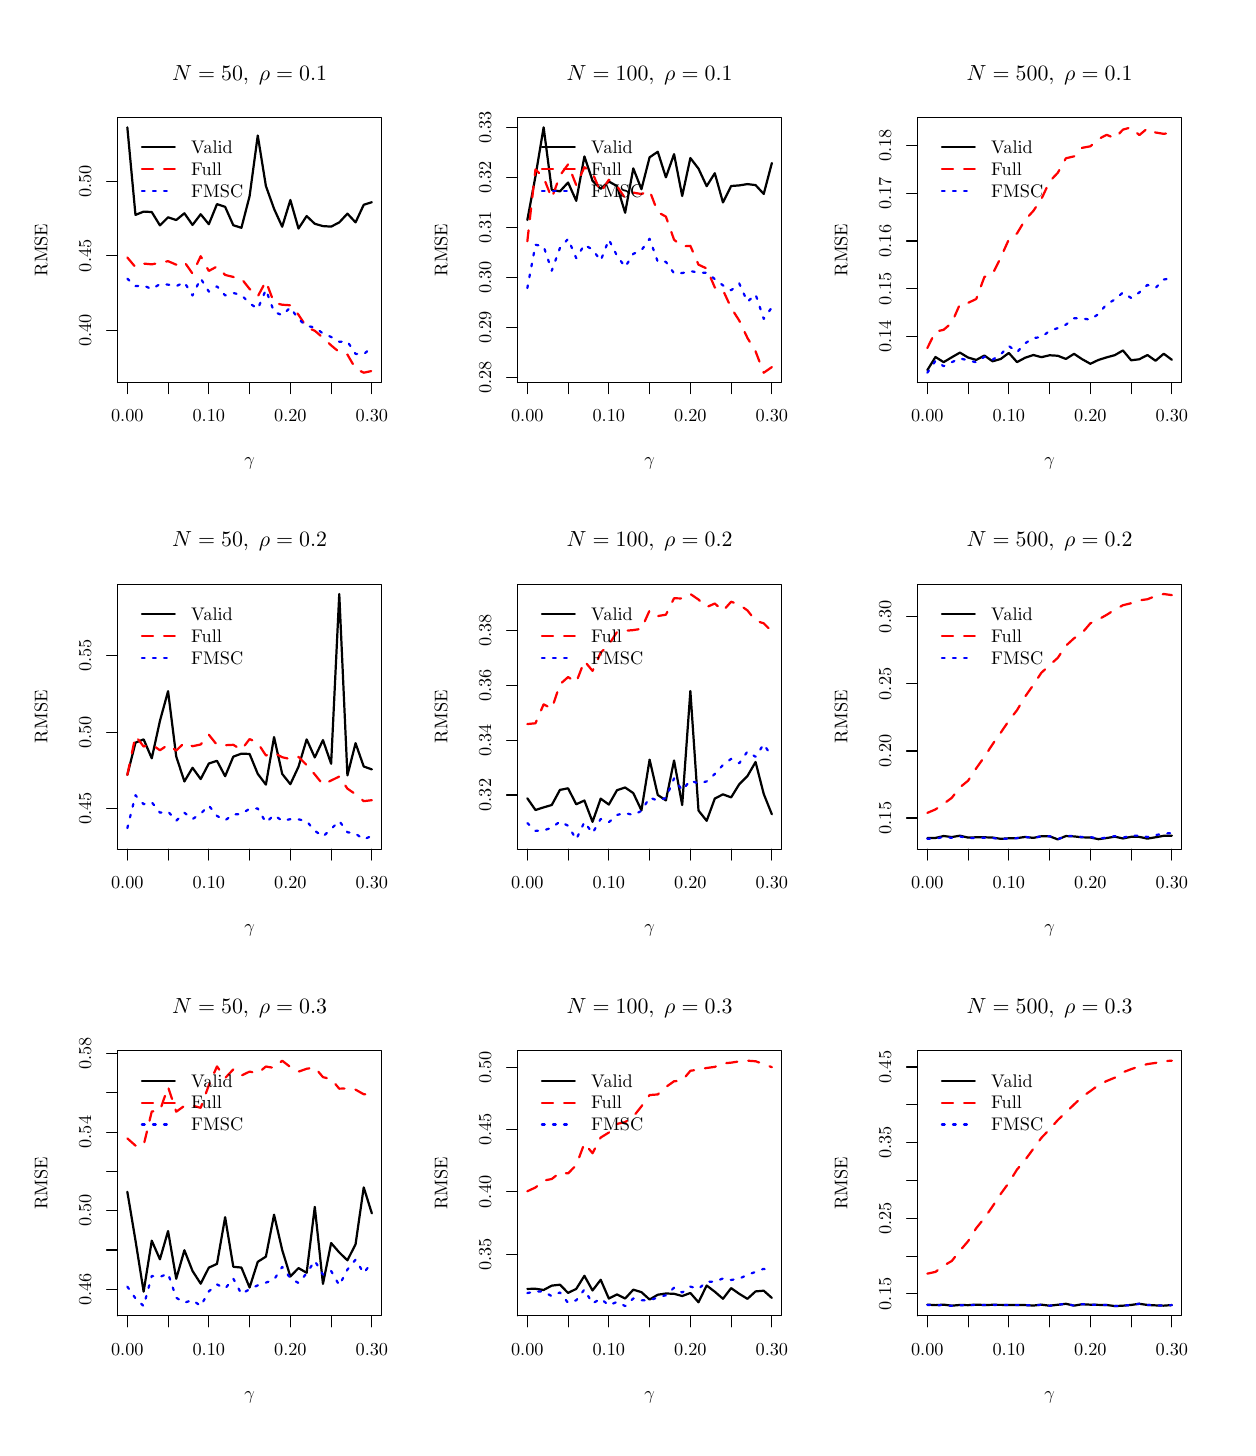
\begin{tikzpicture}[x=1pt,y=1pt]
\definecolor[named]{fillColor}{rgb}{1.00,1.00,1.00}
\path[use as bounding box,fill=fillColor,fill opacity=0.00] (0,0) rectangle (433.62,505.89);
\begin{scope}
\path[clip] ( 32.47,377.65) rectangle (127.91,473.42);
\definecolor[named]{drawColor}{rgb}{0.00,0.00,0.00}

\path[draw=drawColor,line width= 0.8pt,line join=round,line cap=round] ( 36.01,469.87) --
	( 38.95,438.24) --
	( 41.90,439.42) --
	( 44.84,439.26) --
	( 47.79,434.44) --
	( 50.73,437.37) --
	( 53.68,436.38) --
	( 56.63,438.81) --
	( 59.57,434.60) --
	( 62.52,438.47) --
	( 65.46,434.86) --
	( 68.41,442.13) --
	( 71.35,441.13) --
	( 74.30,434.49) --
	( 77.24,433.57) --
	( 80.19,445.01) --
	( 83.14,466.93) --
	( 86.08,448.67) --
	( 89.03,440.43) --
	( 91.97,433.96) --
	( 94.92,443.62) --
	( 97.86,433.31) --
	(100.81,437.81) --
	(103.75,435.02) --
	(106.70,434.18) --
	(109.65,434.00) --
	(112.59,435.51) --
	(115.54,438.69) --
	(118.48,435.52) --
	(121.43,441.89) --
	(124.37,442.82);
\end{scope}
\begin{scope}
\path[clip] (  0.00,  0.00) rectangle (433.62,505.89);
\definecolor[named]{drawColor}{rgb}{0.00,0.00,0.00}

\path[draw=drawColor,line width= 0.4pt,line join=round,line cap=round] ( 36.01,377.65) -- (124.37,377.65);

\path[draw=drawColor,line width= 0.4pt,line join=round,line cap=round] ( 36.01,377.65) -- ( 36.01,373.69);

\path[draw=drawColor,line width= 0.4pt,line join=round,line cap=round] ( 50.73,377.65) -- ( 50.73,373.69);

\path[draw=drawColor,line width= 0.4pt,line join=round,line cap=round] ( 65.46,377.65) -- ( 65.46,373.69);

\path[draw=drawColor,line width= 0.4pt,line join=round,line cap=round] ( 80.19,377.65) -- ( 80.19,373.69);

\path[draw=drawColor,line width= 0.4pt,line join=round,line cap=round] ( 94.92,377.65) -- ( 94.92,373.69);

\path[draw=drawColor,line width= 0.4pt,line join=round,line cap=round] (109.65,377.65) -- (109.65,373.69);

\path[draw=drawColor,line width= 0.4pt,line join=round,line cap=round] (124.37,377.65) -- (124.37,373.69);

\node[text=drawColor,anchor=base,inner sep=0pt, outer sep=0pt, scale=  0.66] at ( 36.01,363.40) {0.00};

\node[text=drawColor,anchor=base,inner sep=0pt, outer sep=0pt, scale=  0.66] at ( 65.46,363.40) {0.10};

\node[text=drawColor,anchor=base,inner sep=0pt, outer sep=0pt, scale=  0.66] at ( 94.92,363.40) {0.20};

\node[text=drawColor,anchor=base,inner sep=0pt, outer sep=0pt, scale=  0.66] at (124.37,363.40) {0.30};

\path[draw=drawColor,line width= 0.4pt,line join=round,line cap=round] ( 32.47,396.54) -- ( 32.47,450.39);

\path[draw=drawColor,line width= 0.4pt,line join=round,line cap=round] ( 32.47,396.54) -- ( 28.51,396.54);

\path[draw=drawColor,line width= 0.4pt,line join=round,line cap=round] ( 32.47,423.46) -- ( 28.51,423.46);

\path[draw=drawColor,line width= 0.4pt,line join=round,line cap=round] ( 32.47,450.39) -- ( 28.51,450.39);

\node[text=drawColor,rotate= 90.00,anchor=base,inner sep=0pt, outer sep=0pt, scale=  0.66] at ( 22.97,396.54) {0.40};

\node[text=drawColor,rotate= 90.00,anchor=base,inner sep=0pt, outer sep=0pt, scale=  0.66] at ( 22.97,423.46) {0.45};

\node[text=drawColor,rotate= 90.00,anchor=base,inner sep=0pt, outer sep=0pt, scale=  0.66] at ( 22.97,450.39) {0.50};

\path[draw=drawColor,line width= 0.4pt,line join=round,line cap=round] ( 32.47,377.65) --
	(127.91,377.65) --
	(127.91,473.42) --
	( 32.47,473.42) --
	( 32.47,377.65);
\end{scope}
\begin{scope}
\path[clip] (  0.00,337.26) rectangle (144.54,505.89);
\definecolor[named]{drawColor}{rgb}{0.00,0.00,0.00}

\node[text=drawColor,anchor=base,inner sep=0pt, outer sep=0pt, scale=  0.79] at ( 80.19,486.92) {\bfseries $N=50, \;\rho=0.1$};

\node[text=drawColor,anchor=base,inner sep=0pt, outer sep=0pt, scale=  0.66] at ( 80.19,347.56) {$\gamma$};

\node[text=drawColor,rotate= 90.00,anchor=base,inner sep=0pt, outer sep=0pt, scale=  0.66] at (  7.13,425.53) {RMSE};
\end{scope}
\begin{scope}
\path[clip] ( 32.47,377.65) rectangle (127.91,473.42);
\definecolor[named]{drawColor}{rgb}{1.00,0.00,0.00}

\path[draw=drawColor,line width= 0.8pt,dash pattern=on 4pt off 4pt ,line join=round,line cap=round] ( 36.01,422.84) --
	( 38.95,419.35) --
	( 41.90,420.63) --
	( 44.84,420.37) --
	( 47.79,420.92) --
	( 50.73,421.51) --
	( 53.68,420.24) --
	( 56.63,421.24) --
	( 59.57,417.02) --
	( 62.52,423.30) --
	( 65.46,417.98) --
	( 68.41,419.59) --
	( 71.35,416.53) --
	( 74.30,415.81) --
	( 77.24,415.20) --
	( 80.19,411.48) --
	( 83.14,408.77) --
	( 86.08,414.25) --
	( 89.03,406.46) --
	( 91.97,405.77) --
	( 94.92,405.57) --
	( 97.86,402.16) --
	(100.81,397.64) --
	(103.75,396.36) --
	(106.70,393.85) --
	(109.65,391.09) --
	(112.59,388.64) --
	(115.54,387.75) --
	(118.48,382.70) --
	(121.43,381.20) --
	(124.37,381.84);
\definecolor[named]{drawColor}{rgb}{0.00,0.00,1.00}

\path[draw=drawColor,line width= 0.8pt,dash pattern=on 1pt off 3pt ,line join=round,line cap=round] ( 36.01,415.20) --
	( 38.95,412.50) --
	( 41.90,412.72) --
	( 44.84,411.42) --
	( 47.79,413.23) --
	( 50.73,413.03) --
	( 53.68,412.47) --
	( 56.63,413.89) --
	( 59.57,409.12) --
	( 62.52,415.25) --
	( 65.46,410.52) --
	( 68.41,412.41) --
	( 71.35,409.14) --
	( 74.30,410.03) --
	( 77.24,409.24) --
	( 80.19,406.31) --
	( 83.14,404.27) --
	( 86.08,411.18) --
	( 89.03,403.23) --
	( 91.97,401.97) --
	( 94.92,404.78) --
	( 97.86,400.56) --
	(100.81,398.08) --
	(103.75,397.59) --
	(106.70,395.38) --
	(109.65,394.13) --
	(112.59,392.41) --
	(115.54,392.46) --
	(118.48,388.01) --
	(121.43,387.91) --
	(124.37,390.35);
\definecolor[named]{drawColor}{rgb}{0.00,0.00,0.00}

\path[draw=drawColor,line width= 0.8pt,line join=round,line cap=round] ( 41.28,462.63) -- ( 53.16,462.63);
\definecolor[named]{drawColor}{rgb}{1.00,0.00,0.00}

\path[draw=drawColor,line width= 0.8pt,dash pattern=on 4pt off 4pt ,line join=round,line cap=round] ( 41.28,454.71) -- ( 53.16,454.71);
\definecolor[named]{drawColor}{rgb}{0.00,0.00,1.00}

\path[draw=drawColor,line width= 0.8pt,dash pattern=on 1pt off 3pt ,line join=round,line cap=round] ( 41.28,446.79) -- ( 53.16,446.79);
\definecolor[named]{drawColor}{rgb}{0.00,0.00,0.00}

\node[text=drawColor,anchor=base west,inner sep=0pt, outer sep=0pt, scale=  0.66] at ( 59.10,460.35) {Valid};

\node[text=drawColor,anchor=base west,inner sep=0pt, outer sep=0pt, scale=  0.66] at ( 59.10,452.43) {Full};

\node[text=drawColor,anchor=base west,inner sep=0pt, outer sep=0pt, scale=  0.66] at ( 59.10,444.51) {FMSC};
\end{scope}
\begin{scope}
\path[clip] (177.01,377.65) rectangle (272.45,473.42);
\definecolor[named]{drawColor}{rgb}{0.00,0.00,0.00}

\path[draw=drawColor,line width= 0.8pt,line join=round,line cap=round] (180.55,436.38) --
	(183.49,452.19) --
	(186.44,469.87) --
	(189.38,447.26) --
	(192.33,446.74) --
	(195.27,449.93) --
	(198.22,443.33) --
	(201.17,459.36) --
	(204.11,450.53) --
	(207.06,447.67) --
	(210.00,450.30) --
	(212.95,448.65) --
	(215.89,439.02) --
	(218.84,455.03) --
	(221.78,447.52) --
	(224.73,459.04) --
	(227.68,461.05) --
	(230.62,451.80) --
	(233.57,460.19) --
	(236.51,445.06) --
	(239.46,458.78) --
	(242.40,454.95) --
	(245.35,448.62) --
	(248.29,453.29) --
	(251.24,442.73) --
	(254.19,448.67) --
	(257.13,448.89) --
	(260.08,449.36) --
	(263.02,449.00) --
	(265.97,445.80) --
	(268.91,456.97);
\end{scope}
\begin{scope}
\path[clip] (  0.00,  0.00) rectangle (433.62,505.89);
\definecolor[named]{drawColor}{rgb}{0.00,0.00,0.00}

\path[draw=drawColor,line width= 0.4pt,line join=round,line cap=round] (180.55,377.65) -- (268.91,377.65);

\path[draw=drawColor,line width= 0.4pt,line join=round,line cap=round] (180.55,377.65) -- (180.55,373.69);

\path[draw=drawColor,line width= 0.4pt,line join=round,line cap=round] (195.27,377.65) -- (195.27,373.69);

\path[draw=drawColor,line width= 0.4pt,line join=round,line cap=round] (210.00,377.65) -- (210.00,373.69);

\path[draw=drawColor,line width= 0.4pt,line join=round,line cap=round] (224.73,377.65) -- (224.73,373.69);

\path[draw=drawColor,line width= 0.4pt,line join=round,line cap=round] (239.46,377.65) -- (239.46,373.69);

\path[draw=drawColor,line width= 0.4pt,line join=round,line cap=round] (254.19,377.65) -- (254.19,373.69);

\path[draw=drawColor,line width= 0.4pt,line join=round,line cap=round] (268.91,377.65) -- (268.91,373.69);

\node[text=drawColor,anchor=base,inner sep=0pt, outer sep=0pt, scale=  0.66] at (180.55,363.40) {0.00};

\node[text=drawColor,anchor=base,inner sep=0pt, outer sep=0pt, scale=  0.66] at (210.00,363.40) {0.10};

\node[text=drawColor,anchor=base,inner sep=0pt, outer sep=0pt, scale=  0.66] at (239.46,363.40) {0.20};

\node[text=drawColor,anchor=base,inner sep=0pt, outer sep=0pt, scale=  0.66] at (268.91,363.40) {0.30};

\path[draw=drawColor,line width= 0.4pt,line join=round,line cap=round] (177.01,379.47) -- (177.01,469.73);

\path[draw=drawColor,line width= 0.4pt,line join=round,line cap=round] (177.01,379.47) -- (173.05,379.47);

\path[draw=drawColor,line width= 0.4pt,line join=round,line cap=round] (177.01,397.52) -- (173.05,397.52);

\path[draw=drawColor,line width= 0.4pt,line join=round,line cap=round] (177.01,415.58) -- (173.05,415.58);

\path[draw=drawColor,line width= 0.4pt,line join=round,line cap=round] (177.01,433.63) -- (173.05,433.63);

\path[draw=drawColor,line width= 0.4pt,line join=round,line cap=round] (177.01,451.68) -- (173.05,451.68);

\path[draw=drawColor,line width= 0.4pt,line join=round,line cap=round] (177.01,469.73) -- (173.05,469.73);

\node[text=drawColor,rotate= 90.00,anchor=base,inner sep=0pt, outer sep=0pt, scale=  0.66] at (167.51,379.47) {0.28};

\node[text=drawColor,rotate= 90.00,anchor=base,inner sep=0pt, outer sep=0pt, scale=  0.66] at (167.51,397.52) {0.29};

\node[text=drawColor,rotate= 90.00,anchor=base,inner sep=0pt, outer sep=0pt, scale=  0.66] at (167.51,415.58) {0.30};

\node[text=drawColor,rotate= 90.00,anchor=base,inner sep=0pt, outer sep=0pt, scale=  0.66] at (167.51,433.63) {0.31};

\node[text=drawColor,rotate= 90.00,anchor=base,inner sep=0pt, outer sep=0pt, scale=  0.66] at (167.51,451.68) {0.32};

\node[text=drawColor,rotate= 90.00,anchor=base,inner sep=0pt, outer sep=0pt, scale=  0.66] at (167.51,469.73) {0.33};

\path[draw=drawColor,line width= 0.4pt,line join=round,line cap=round] (177.01,377.65) --
	(272.45,377.65) --
	(272.45,473.42) --
	(177.01,473.42) --
	(177.01,377.65);
\end{scope}
\begin{scope}
\path[clip] (144.54,337.26) rectangle (289.08,505.89);
\definecolor[named]{drawColor}{rgb}{0.00,0.00,0.00}

\node[text=drawColor,anchor=base,inner sep=0pt, outer sep=0pt, scale=  0.79] at (224.73,486.92) {\bfseries $N=100, \;\rho=0.1$};

\node[text=drawColor,anchor=base,inner sep=0pt, outer sep=0pt, scale=  0.66] at (224.73,347.56) {$\gamma$};

\node[text=drawColor,rotate= 90.00,anchor=base,inner sep=0pt, outer sep=0pt, scale=  0.66] at (151.67,425.53) {RMSE};
\end{scope}
\begin{scope}
\path[clip] (177.01,377.65) rectangle (272.45,473.42);
\definecolor[named]{drawColor}{rgb}{1.00,0.00,0.00}

\path[draw=drawColor,line width= 0.8pt,dash pattern=on 4pt off 4pt ,line join=round,line cap=round] (180.55,428.69) --
	(183.49,454.68) --
	(186.44,451.70) --
	(189.38,444.28) --
	(192.33,452.45) --
	(195.27,456.48) --
	(198.22,449.01) --
	(201.17,455.46) --
	(204.11,453.37) --
	(207.06,446.42) --
	(210.00,450.92) --
	(212.95,448.63) --
	(215.89,444.23) --
	(218.84,446.28) --
	(221.78,445.77) --
	(224.73,446.98) --
	(227.68,439.24) --
	(230.62,437.61) --
	(233.57,429.26) --
	(236.51,426.86) --
	(239.46,427.05) --
	(242.40,420.25) --
	(245.35,418.87) --
	(248.29,412.01) --
	(251.24,411.05) --
	(254.19,404.64) --
	(257.13,400.04) --
	(260.08,393.78) --
	(263.02,388.93) --
	(265.97,381.20) --
	(268.91,383.23);
\definecolor[named]{drawColor}{rgb}{0.00,0.00,1.00}

\path[draw=drawColor,line width= 0.8pt,dash pattern=on 1pt off 3pt ,line join=round,line cap=round] (180.55,411.78) --
	(183.49,427.44) --
	(186.44,426.88) --
	(189.38,418.08) --
	(192.33,426.27) --
	(195.27,429.57) --
	(198.22,422.61) --
	(201.17,427.44) --
	(204.11,425.67) --
	(207.06,421.71) --
	(210.00,429.31) --
	(212.95,423.48) --
	(215.89,419.39) --
	(218.84,424.15) --
	(221.78,425.45) --
	(224.73,429.61) --
	(227.68,421.30) --
	(230.62,421.27) --
	(233.57,417.11) --
	(236.51,417.21) --
	(239.46,417.94) --
	(242.40,417.38) --
	(245.35,417.30) --
	(248.29,415.05) --
	(251.24,412.76) --
	(254.19,410.99) --
	(257.13,413.44) --
	(260.08,406.83) --
	(263.02,409.52) --
	(265.97,400.65) --
	(268.91,404.84);
\definecolor[named]{drawColor}{rgb}{0.00,0.00,0.00}

\path[draw=drawColor,line width= 0.8pt,line join=round,line cap=round] (185.82,462.63) -- (197.70,462.63);
\definecolor[named]{drawColor}{rgb}{1.00,0.00,0.00}

\path[draw=drawColor,line width= 0.8pt,dash pattern=on 4pt off 4pt ,line join=round,line cap=round] (185.82,454.71) -- (197.70,454.71);
\definecolor[named]{drawColor}{rgb}{0.00,0.00,1.00}

\path[draw=drawColor,line width= 0.8pt,dash pattern=on 1pt off 3pt ,line join=round,line cap=round] (185.82,446.79) -- (197.70,446.79);
\definecolor[named]{drawColor}{rgb}{0.00,0.00,0.00}

\node[text=drawColor,anchor=base west,inner sep=0pt, outer sep=0pt, scale=  0.66] at (203.64,460.35) {Valid};

\node[text=drawColor,anchor=base west,inner sep=0pt, outer sep=0pt, scale=  0.66] at (203.64,452.43) {Full};

\node[text=drawColor,anchor=base west,inner sep=0pt, outer sep=0pt, scale=  0.66] at (203.64,444.51) {FMSC};
\end{scope}
\begin{scope}
\path[clip] (321.55,377.65) rectangle (416.99,473.42);
\definecolor[named]{drawColor}{rgb}{0.00,0.00,0.00}

\path[draw=drawColor,line width= 0.8pt,line join=round,line cap=round] (325.09,382.14) --
	(328.03,386.88) --
	(330.98,385.02) --
	(333.92,386.78) --
	(336.87,388.47) --
	(339.81,386.69) --
	(342.76,385.83) --
	(345.71,387.41) --
	(348.65,385.33) --
	(351.60,386.16) --
	(354.54,388.35) --
	(357.49,385.04) --
	(360.43,386.61) --
	(363.38,387.61) --
	(366.32,386.82) --
	(369.27,387.51) --
	(372.22,387.33) --
	(375.16,386.18) --
	(378.11,388.03) --
	(381.05,386.08) --
	(384.00,384.43) --
	(386.94,385.83) --
	(389.89,386.75) --
	(392.83,387.55) --
	(395.78,389.25) --
	(398.73,385.70) --
	(401.67,386.06) --
	(404.62,387.60) --
	(407.56,385.53) --
	(410.51,388.06) --
	(413.45,385.88);
\end{scope}
\begin{scope}
\path[clip] (  0.00,  0.00) rectangle (433.62,505.89);
\definecolor[named]{drawColor}{rgb}{0.00,0.00,0.00}

\path[draw=drawColor,line width= 0.4pt,line join=round,line cap=round] (325.09,377.65) -- (413.45,377.65);

\path[draw=drawColor,line width= 0.4pt,line join=round,line cap=round] (325.09,377.65) -- (325.09,373.69);

\path[draw=drawColor,line width= 0.4pt,line join=round,line cap=round] (339.81,377.65) -- (339.81,373.69);

\path[draw=drawColor,line width= 0.4pt,line join=round,line cap=round] (354.54,377.65) -- (354.54,373.69);

\path[draw=drawColor,line width= 0.4pt,line join=round,line cap=round] (369.27,377.65) -- (369.27,373.69);

\path[draw=drawColor,line width= 0.4pt,line join=round,line cap=round] (384.00,377.65) -- (384.00,373.69);

\path[draw=drawColor,line width= 0.4pt,line join=round,line cap=round] (398.73,377.65) -- (398.73,373.69);

\path[draw=drawColor,line width= 0.4pt,line join=round,line cap=round] (413.45,377.65) -- (413.45,373.69);

\node[text=drawColor,anchor=base,inner sep=0pt, outer sep=0pt, scale=  0.66] at (325.09,363.40) {0.00};

\node[text=drawColor,anchor=base,inner sep=0pt, outer sep=0pt, scale=  0.66] at (354.54,363.40) {0.10};

\node[text=drawColor,anchor=base,inner sep=0pt, outer sep=0pt, scale=  0.66] at (384.00,363.40) {0.20};

\node[text=drawColor,anchor=base,inner sep=0pt, outer sep=0pt, scale=  0.66] at (413.45,363.40) {0.30};

\path[draw=drawColor,line width= 0.4pt,line join=round,line cap=round] (321.55,394.25) -- (321.55,463.36);

\path[draw=drawColor,line width= 0.4pt,line join=round,line cap=round] (321.55,394.25) -- (317.59,394.25);

\path[draw=drawColor,line width= 0.4pt,line join=round,line cap=round] (321.55,411.53) -- (317.59,411.53);

\path[draw=drawColor,line width= 0.4pt,line join=round,line cap=round] (321.55,428.81) -- (317.59,428.81);

\path[draw=drawColor,line width= 0.4pt,line join=round,line cap=round] (321.55,446.09) -- (317.59,446.09);

\path[draw=drawColor,line width= 0.4pt,line join=round,line cap=round] (321.55,463.36) -- (317.59,463.36);

\node[text=drawColor,rotate= 90.00,anchor=base,inner sep=0pt, outer sep=0pt, scale=  0.66] at (312.05,394.25) {0.14};

\node[text=drawColor,rotate= 90.00,anchor=base,inner sep=0pt, outer sep=0pt, scale=  0.66] at (312.05,411.53) {0.15};

\node[text=drawColor,rotate= 90.00,anchor=base,inner sep=0pt, outer sep=0pt, scale=  0.66] at (312.05,428.81) {0.16};

\node[text=drawColor,rotate= 90.00,anchor=base,inner sep=0pt, outer sep=0pt, scale=  0.66] at (312.05,446.09) {0.17};

\node[text=drawColor,rotate= 90.00,anchor=base,inner sep=0pt, outer sep=0pt, scale=  0.66] at (312.05,463.36) {0.18};

\path[draw=drawColor,line width= 0.4pt,line join=round,line cap=round] (321.55,377.65) --
	(416.99,377.65) --
	(416.99,473.42) --
	(321.55,473.42) --
	(321.55,377.65);
\end{scope}
\begin{scope}
\path[clip] (289.08,337.26) rectangle (433.62,505.89);
\definecolor[named]{drawColor}{rgb}{0.00,0.00,0.00}

\node[text=drawColor,anchor=base,inner sep=0pt, outer sep=0pt, scale=  0.79] at (369.27,486.92) {\bfseries $N=500, \;\rho=0.1$};

\node[text=drawColor,anchor=base,inner sep=0pt, outer sep=0pt, scale=  0.66] at (369.27,347.56) {$\gamma$};

\node[text=drawColor,rotate= 90.00,anchor=base,inner sep=0pt, outer sep=0pt, scale=  0.66] at (296.21,425.53) {RMSE};
\end{scope}
\begin{scope}
\path[clip] (321.55,377.65) rectangle (416.99,473.42);
\definecolor[named]{drawColor}{rgb}{1.00,0.00,0.00}

\path[draw=drawColor,line width= 0.8pt,dash pattern=on 4pt off 4pt ,line join=round,line cap=round] (325.09,390.11) --
	(328.03,396.04) --
	(330.98,396.71) --
	(333.92,399.24) --
	(336.87,405.98) --
	(339.81,406.45) --
	(342.76,407.83) --
	(345.71,415.83) --
	(348.65,416.84) --
	(351.60,422.79) --
	(354.54,429.37) --
	(357.49,431.53) --
	(360.43,436.42) --
	(363.38,439.66) --
	(366.32,443.99) --
	(369.27,450.33) --
	(372.22,453.43) --
	(375.16,458.69) --
	(378.11,459.39) --
	(381.05,462.47) --
	(384.00,463.01) --
	(386.94,465.63) --
	(389.89,467.17) --
	(392.83,465.91) --
	(395.78,469.05) --
	(398.73,469.87) --
	(401.67,467.05) --
	(404.62,469.50) --
	(407.56,468.00) --
	(410.51,467.52) --
	(413.45,467.93);
\definecolor[named]{drawColor}{rgb}{0.00,0.00,1.00}

\path[draw=drawColor,line width= 0.8pt,dash pattern=on 1pt off 3pt ,line join=round,line cap=round] (325.09,381.20) --
	(328.03,385.47) --
	(330.98,383.57) --
	(333.92,385.00) --
	(336.87,386.36) --
	(339.81,385.68) --
	(342.76,384.97) --
	(345.71,386.96) --
	(348.65,385.89) --
	(351.60,387.81) --
	(354.54,390.88) --
	(357.49,388.63) --
	(360.43,391.82) --
	(363.38,393.74) --
	(366.32,394.06) --
	(369.27,396.33) --
	(372.22,397.31) --
	(375.16,398.57) --
	(378.11,400.88) --
	(381.05,400.80) --
	(384.00,400.39) --
	(386.94,402.42) --
	(389.89,406.00) --
	(392.83,407.63) --
	(395.78,410.21) --
	(398.73,408.20) --
	(401.67,410.19) --
	(404.62,412.94) --
	(407.56,411.85) --
	(410.51,414.89) --
	(413.45,415.34);
\definecolor[named]{drawColor}{rgb}{0.00,0.00,0.00}

\path[draw=drawColor,line width= 0.8pt,line join=round,line cap=round] (330.36,462.63) -- (342.24,462.63);
\definecolor[named]{drawColor}{rgb}{1.00,0.00,0.00}

\path[draw=drawColor,line width= 0.8pt,dash pattern=on 4pt off 4pt ,line join=round,line cap=round] (330.36,454.71) -- (342.24,454.71);
\definecolor[named]{drawColor}{rgb}{0.00,0.00,1.00}

\path[draw=drawColor,line width= 0.8pt,dash pattern=on 1pt off 3pt ,line join=round,line cap=round] (330.36,446.79) -- (342.24,446.79);
\definecolor[named]{drawColor}{rgb}{0.00,0.00,0.00}

\node[text=drawColor,anchor=base west,inner sep=0pt, outer sep=0pt, scale=  0.66] at (348.18,460.35) {Valid};

\node[text=drawColor,anchor=base west,inner sep=0pt, outer sep=0pt, scale=  0.66] at (348.18,452.43) {Full};

\node[text=drawColor,anchor=base west,inner sep=0pt, outer sep=0pt, scale=  0.66] at (348.18,444.51) {FMSC};
\end{scope}
\begin{scope}
\path[clip] ( 32.47,209.02) rectangle (127.91,304.79);
\definecolor[named]{drawColor}{rgb}{0.00,0.00,0.00}

\path[draw=drawColor,line width= 0.8pt,line join=round,line cap=round] ( 36.01,235.87) --
	( 38.95,247.52) --
	( 41.90,248.72) --
	( 44.84,241.87) --
	( 47.79,255.38) --
	( 50.73,266.12) --
	( 53.68,242.55) --
	( 56.63,233.51) --
	( 59.57,238.45) --
	( 62.52,234.37) --
	( 65.46,240.00) --
	( 68.41,240.96) --
	( 71.35,235.40) --
	( 74.30,242.47) --
	( 77.24,243.56) --
	( 80.19,243.44) --
	( 83.14,236.25) --
	( 86.08,232.37) --
	( 89.03,249.54) --
	( 91.97,236.24) --
	( 94.92,232.52) --
	( 97.86,238.82) --
	(100.81,248.71) --
	(103.75,242.19) --
	(106.70,248.46) --
	(109.65,239.91) --
	(112.59,301.24) --
	(115.54,235.68) --
	(118.48,247.34) --
	(121.43,238.91) --
	(124.37,237.86);
\end{scope}
\begin{scope}
\path[clip] (  0.00,  0.00) rectangle (433.62,505.89);
\definecolor[named]{drawColor}{rgb}{0.00,0.00,0.00}

\path[draw=drawColor,line width= 0.4pt,line join=round,line cap=round] ( 36.01,209.02) -- (124.37,209.02);

\path[draw=drawColor,line width= 0.4pt,line join=round,line cap=round] ( 36.01,209.02) -- ( 36.01,205.06);

\path[draw=drawColor,line width= 0.4pt,line join=round,line cap=round] ( 50.73,209.02) -- ( 50.73,205.06);

\path[draw=drawColor,line width= 0.4pt,line join=round,line cap=round] ( 65.46,209.02) -- ( 65.46,205.06);

\path[draw=drawColor,line width= 0.4pt,line join=round,line cap=round] ( 80.19,209.02) -- ( 80.19,205.06);

\path[draw=drawColor,line width= 0.4pt,line join=round,line cap=round] ( 94.92,209.02) -- ( 94.92,205.06);

\path[draw=drawColor,line width= 0.4pt,line join=round,line cap=round] (109.65,209.02) -- (109.65,205.06);

\path[draw=drawColor,line width= 0.4pt,line join=round,line cap=round] (124.37,209.02) -- (124.37,205.06);

\node[text=drawColor,anchor=base,inner sep=0pt, outer sep=0pt, scale=  0.66] at ( 36.01,194.77) {0.00};

\node[text=drawColor,anchor=base,inner sep=0pt, outer sep=0pt, scale=  0.66] at ( 65.46,194.77) {0.10};

\node[text=drawColor,anchor=base,inner sep=0pt, outer sep=0pt, scale=  0.66] at ( 94.92,194.77) {0.20};

\node[text=drawColor,anchor=base,inner sep=0pt, outer sep=0pt, scale=  0.66] at (124.37,194.77) {0.30};

\path[draw=drawColor,line width= 0.4pt,line join=round,line cap=round] ( 32.47,223.66) -- ( 32.47,278.98);

\path[draw=drawColor,line width= 0.4pt,line join=round,line cap=round] ( 32.47,223.66) -- ( 28.51,223.66);

\path[draw=drawColor,line width= 0.4pt,line join=round,line cap=round] ( 32.47,251.32) -- ( 28.51,251.32);

\path[draw=drawColor,line width= 0.4pt,line join=round,line cap=round] ( 32.47,278.98) -- ( 28.51,278.98);

\node[text=drawColor,rotate= 90.00,anchor=base,inner sep=0pt, outer sep=0pt, scale=  0.66] at ( 22.97,223.66) {0.45};

\node[text=drawColor,rotate= 90.00,anchor=base,inner sep=0pt, outer sep=0pt, scale=  0.66] at ( 22.97,251.32) {0.50};

\node[text=drawColor,rotate= 90.00,anchor=base,inner sep=0pt, outer sep=0pt, scale=  0.66] at ( 22.97,278.98) {0.55};

\path[draw=drawColor,line width= 0.4pt,line join=round,line cap=round] ( 32.47,209.02) --
	(127.91,209.02) --
	(127.91,304.79) --
	( 32.47,304.79) --
	( 32.47,209.02);
\end{scope}
\begin{scope}
\path[clip] (  0.00,168.63) rectangle (144.54,337.26);
\definecolor[named]{drawColor}{rgb}{0.00,0.00,0.00}

\node[text=drawColor,anchor=base,inner sep=0pt, outer sep=0pt, scale=  0.79] at ( 80.19,318.29) {\bfseries $N=50, \;\rho=0.2$};

\node[text=drawColor,anchor=base,inner sep=0pt, outer sep=0pt, scale=  0.66] at ( 80.19,178.93) {$\gamma$};

\node[text=drawColor,rotate= 90.00,anchor=base,inner sep=0pt, outer sep=0pt, scale=  0.66] at (  7.13,256.90) {RMSE};
\end{scope}
\begin{scope}
\path[clip] ( 32.47,209.02) rectangle (127.91,304.79);
\definecolor[named]{drawColor}{rgb}{1.00,0.00,0.00}

\path[draw=drawColor,line width= 0.8pt,dash pattern=on 4pt off 4pt ,line join=round,line cap=round] ( 36.01,235.84) --
	( 38.95,249.97) --
	( 41.90,246.14) --
	( 44.84,246.85) --
	( 47.79,244.79) --
	( 50.73,246.76) --
	( 53.68,244.66) --
	( 56.63,247.53) --
	( 59.57,246.24) --
	( 62.52,246.87) --
	( 65.46,250.40) --
	( 68.41,246.71) --
	( 71.35,246.60) --
	( 74.30,246.75) --
	( 77.24,244.95) --
	( 80.19,248.83) --
	( 83.14,247.41) --
	( 86.08,242.90) --
	( 89.03,243.86) --
	( 91.97,242.26) --
	( 94.92,241.59) --
	( 97.86,242.39) --
	(100.81,239.43) --
	(103.75,236.05) --
	(106.70,232.37) --
	(109.65,233.84) --
	(112.59,235.29) --
	(115.54,230.90) --
	(118.48,228.91) --
	(121.43,226.39) --
	(124.37,226.74);
\definecolor[named]{drawColor}{rgb}{0.00,0.00,1.00}

\path[draw=drawColor,line width= 0.8pt,dash pattern=on 1pt off 3pt ,line join=round,line cap=round] ( 36.01,216.63) --
	( 38.95,228.53) --
	( 41.90,225.29) --
	( 44.84,226.00) --
	( 47.79,222.23) --
	( 50.73,222.63) --
	( 53.68,219.30) --
	( 56.63,222.20) --
	( 59.57,219.91) --
	( 62.52,221.88) --
	( 65.46,224.80) --
	( 68.41,221.05) --
	( 71.35,219.46) --
	( 74.30,221.59) --
	( 77.24,221.75) --
	( 80.19,223.67) --
	( 83.14,223.74) --
	( 86.08,218.69) --
	( 89.03,221.34) --
	( 91.97,219.30) --
	( 94.92,219.87) --
	( 97.86,219.83) --
	(100.81,219.14) --
	(103.75,215.69) --
	(106.70,213.60) --
	(109.65,216.32) --
	(112.59,219.23) --
	(115.54,215.17) --
	(118.48,214.64) --
	(121.43,212.57) --
	(124.37,213.85);
\definecolor[named]{drawColor}{rgb}{0.00,0.00,0.00}

\path[draw=drawColor,line width= 0.8pt,line join=round,line cap=round] ( 41.28,294.00) -- ( 53.16,294.00);
\definecolor[named]{drawColor}{rgb}{1.00,0.00,0.00}

\path[draw=drawColor,line width= 0.8pt,dash pattern=on 4pt off 4pt ,line join=round,line cap=round] ( 41.28,286.08) -- ( 53.16,286.08);
\definecolor[named]{drawColor}{rgb}{0.00,0.00,1.00}

\path[draw=drawColor,line width= 0.8pt,dash pattern=on 1pt off 3pt ,line join=round,line cap=round] ( 41.28,278.16) -- ( 53.16,278.16);
\definecolor[named]{drawColor}{rgb}{0.00,0.00,0.00}

\node[text=drawColor,anchor=base west,inner sep=0pt, outer sep=0pt, scale=  0.66] at ( 59.10,291.72) {Valid};

\node[text=drawColor,anchor=base west,inner sep=0pt, outer sep=0pt, scale=  0.66] at ( 59.10,283.80) {Full};

\node[text=drawColor,anchor=base west,inner sep=0pt, outer sep=0pt, scale=  0.66] at ( 59.10,275.88) {FMSC};
\end{scope}
\begin{scope}
\path[clip] (177.01,209.02) rectangle (272.45,304.79);
\definecolor[named]{drawColor}{rgb}{0.00,0.00,0.00}

\path[draw=drawColor,line width= 0.8pt,line join=round,line cap=round] (180.55,227.43) --
	(183.49,223.19) --
	(186.44,224.14) --
	(189.38,225.00) --
	(192.33,230.46) --
	(195.27,231.04) --
	(198.22,225.26) --
	(201.17,226.62) --
	(204.11,218.91) --
	(207.06,227.29) --
	(210.00,225.16) --
	(212.95,230.35) --
	(215.89,231.33) --
	(218.84,229.29) --
	(221.78,223.08) --
	(224.73,241.40) --
	(227.68,228.64) --
	(230.62,226.65) --
	(233.57,241.09) --
	(236.51,224.98) --
	(239.46,266.19) --
	(242.40,223.00) --
	(245.35,219.29) --
	(248.29,227.32) --
	(251.24,228.85) --
	(254.19,227.75) --
	(257.13,232.51) --
	(260.08,235.45) --
	(263.02,240.55) --
	(265.97,229.00) --
	(268.91,221.64);
\end{scope}
\begin{scope}
\path[clip] (  0.00,  0.00) rectangle (433.62,505.89);
\definecolor[named]{drawColor}{rgb}{0.00,0.00,0.00}

\path[draw=drawColor,line width= 0.4pt,line join=round,line cap=round] (180.55,209.02) -- (268.91,209.02);

\path[draw=drawColor,line width= 0.4pt,line join=round,line cap=round] (180.55,209.02) -- (180.55,205.06);

\path[draw=drawColor,line width= 0.4pt,line join=round,line cap=round] (195.27,209.02) -- (195.27,205.06);

\path[draw=drawColor,line width= 0.4pt,line join=round,line cap=round] (210.00,209.02) -- (210.00,205.06);

\path[draw=drawColor,line width= 0.4pt,line join=round,line cap=round] (224.73,209.02) -- (224.73,205.06);

\path[draw=drawColor,line width= 0.4pt,line join=round,line cap=round] (239.46,209.02) -- (239.46,205.06);

\path[draw=drawColor,line width= 0.4pt,line join=round,line cap=round] (254.19,209.02) -- (254.19,205.06);

\path[draw=drawColor,line width= 0.4pt,line join=round,line cap=round] (268.91,209.02) -- (268.91,205.06);

\node[text=drawColor,anchor=base,inner sep=0pt, outer sep=0pt, scale=  0.66] at (180.55,194.77) {0.00};

\node[text=drawColor,anchor=base,inner sep=0pt, outer sep=0pt, scale=  0.66] at (210.00,194.77) {0.10};

\node[text=drawColor,anchor=base,inner sep=0pt, outer sep=0pt, scale=  0.66] at (239.46,194.77) {0.20};

\node[text=drawColor,anchor=base,inner sep=0pt, outer sep=0pt, scale=  0.66] at (268.91,194.77) {0.30};

\path[draw=drawColor,line width= 0.4pt,line join=round,line cap=round] (177.01,228.62) -- (177.01,287.99);

\path[draw=drawColor,line width= 0.4pt,line join=round,line cap=round] (177.01,228.62) -- (173.05,228.62);

\path[draw=drawColor,line width= 0.4pt,line join=round,line cap=round] (177.01,248.41) -- (173.05,248.41);

\path[draw=drawColor,line width= 0.4pt,line join=round,line cap=round] (177.01,268.20) -- (173.05,268.20);

\path[draw=drawColor,line width= 0.4pt,line join=round,line cap=round] (177.01,287.99) -- (173.05,287.99);

\node[text=drawColor,rotate= 90.00,anchor=base,inner sep=0pt, outer sep=0pt, scale=  0.66] at (167.51,228.62) {0.32};

\node[text=drawColor,rotate= 90.00,anchor=base,inner sep=0pt, outer sep=0pt, scale=  0.66] at (167.51,248.41) {0.34};

\node[text=drawColor,rotate= 90.00,anchor=base,inner sep=0pt, outer sep=0pt, scale=  0.66] at (167.51,268.20) {0.36};

\node[text=drawColor,rotate= 90.00,anchor=base,inner sep=0pt, outer sep=0pt, scale=  0.66] at (167.51,287.99) {0.38};

\path[draw=drawColor,line width= 0.4pt,line join=round,line cap=round] (177.01,209.02) --
	(272.45,209.02) --
	(272.45,304.79) --
	(177.01,304.79) --
	(177.01,209.02);
\end{scope}
\begin{scope}
\path[clip] (144.54,168.63) rectangle (289.08,337.26);
\definecolor[named]{drawColor}{rgb}{0.00,0.00,0.00}

\node[text=drawColor,anchor=base,inner sep=0pt, outer sep=0pt, scale=  0.79] at (224.73,318.29) {\bfseries $N=100, \;\rho=0.2$};

\node[text=drawColor,anchor=base,inner sep=0pt, outer sep=0pt, scale=  0.66] at (224.73,178.93) {$\gamma$};

\node[text=drawColor,rotate= 90.00,anchor=base,inner sep=0pt, outer sep=0pt, scale=  0.66] at (151.67,256.90) {RMSE};
\end{scope}
\begin{scope}
\path[clip] (177.01,209.02) rectangle (272.45,304.79);
\definecolor[named]{drawColor}{rgb}{1.00,0.00,0.00}

\path[draw=drawColor,line width= 0.8pt,dash pattern=on 4pt off 4pt ,line join=round,line cap=round] (180.55,254.25) --
	(183.49,254.53) --
	(186.44,261.38) --
	(189.38,259.81) --
	(192.33,268.60) --
	(195.27,271.23) --
	(198.22,269.36) --
	(201.17,277.04) --
	(204.11,273.45) --
	(207.06,280.04) --
	(210.00,282.92) --
	(212.95,287.51) --
	(215.89,287.95) --
	(218.84,288.20) --
	(221.78,288.67) --
	(224.73,295.29) --
	(227.68,293.27) --
	(230.62,293.76) --
	(233.57,299.70) --
	(236.51,299.63) --
	(239.46,301.24) --
	(242.40,299.24) --
	(245.35,296.51) --
	(248.29,297.81) --
	(251.24,295.13) --
	(254.19,298.45) --
	(257.13,297.42) --
	(260.08,295.31) --
	(263.02,291.61) --
	(265.97,290.65) --
	(268.91,287.68);
\definecolor[named]{drawColor}{rgb}{0.00,0.00,1.00}

\path[draw=drawColor,line width= 0.8pt,dash pattern=on 1pt off 3pt ,line join=round,line cap=round] (180.55,218.48) --
	(183.49,215.65) --
	(186.44,215.81) --
	(189.38,216.78) --
	(192.33,219.03) --
	(195.27,217.51) --
	(198.22,212.57) --
	(201.17,218.86) --
	(204.11,214.81) --
	(207.06,219.96) --
	(210.00,218.77) --
	(212.95,221.40) --
	(215.89,222.11) --
	(218.84,221.37) --
	(221.78,222.87) --
	(224.73,227.69) --
	(227.68,226.58) --
	(230.62,227.52) --
	(233.57,234.60) --
	(236.51,230.33) --
	(239.46,233.88) --
	(242.40,232.73) --
	(245.35,233.54) --
	(248.29,236.21) --
	(251.24,239.45) --
	(254.19,241.66) --
	(257.13,240.09) --
	(260.08,244.31) --
	(263.02,242.42) --
	(265.97,246.99) --
	(268.91,242.49);
\definecolor[named]{drawColor}{rgb}{0.00,0.00,0.00}

\path[draw=drawColor,line width= 0.8pt,line join=round,line cap=round] (185.82,294.00) -- (197.70,294.00);
\definecolor[named]{drawColor}{rgb}{1.00,0.00,0.00}

\path[draw=drawColor,line width= 0.8pt,dash pattern=on 4pt off 4pt ,line join=round,line cap=round] (185.82,286.08) -- (197.70,286.08);
\definecolor[named]{drawColor}{rgb}{0.00,0.00,1.00}

\path[draw=drawColor,line width= 0.8pt,dash pattern=on 1pt off 3pt ,line join=round,line cap=round] (185.82,278.16) -- (197.70,278.16);
\definecolor[named]{drawColor}{rgb}{0.00,0.00,0.00}

\node[text=drawColor,anchor=base west,inner sep=0pt, outer sep=0pt, scale=  0.66] at (203.64,291.72) {Valid};

\node[text=drawColor,anchor=base west,inner sep=0pt, outer sep=0pt, scale=  0.66] at (203.64,283.80) {Full};

\node[text=drawColor,anchor=base west,inner sep=0pt, outer sep=0pt, scale=  0.66] at (203.64,275.88) {FMSC};
\end{scope}
\begin{scope}
\path[clip] (321.55,209.02) rectangle (416.99,304.79);
\definecolor[named]{drawColor}{rgb}{0.00,0.00,0.00}

\path[draw=drawColor,line width= 0.8pt,line join=round,line cap=round] (325.09,213.04) --
	(328.03,213.10) --
	(330.98,213.79) --
	(333.92,213.42) --
	(336.87,213.90) --
	(339.81,213.23) --
	(342.76,213.33) --
	(345.71,213.33) --
	(348.65,213.24) --
	(351.60,212.77) --
	(354.54,212.97) --
	(357.49,213.04) --
	(360.43,213.46) --
	(363.38,213.12) --
	(366.32,213.71) --
	(369.27,213.70) --
	(372.22,212.57) --
	(375.16,213.78) --
	(378.11,213.65) --
	(381.05,213.31) --
	(384.00,213.26) --
	(386.94,212.65) --
	(389.89,213.07) --
	(392.83,213.55) --
	(395.78,212.91) --
	(398.73,213.50) --
	(401.67,213.48) --
	(404.62,212.85) --
	(407.56,213.34) --
	(410.51,213.87) --
	(413.45,213.90);
\end{scope}
\begin{scope}
\path[clip] (  0.00,  0.00) rectangle (433.62,505.89);
\definecolor[named]{drawColor}{rgb}{0.00,0.00,0.00}

\path[draw=drawColor,line width= 0.4pt,line join=round,line cap=round] (325.09,209.02) -- (413.45,209.02);

\path[draw=drawColor,line width= 0.4pt,line join=round,line cap=round] (325.09,209.02) -- (325.09,205.06);

\path[draw=drawColor,line width= 0.4pt,line join=round,line cap=round] (339.81,209.02) -- (339.81,205.06);

\path[draw=drawColor,line width= 0.4pt,line join=round,line cap=round] (354.54,209.02) -- (354.54,205.06);

\path[draw=drawColor,line width= 0.4pt,line join=round,line cap=round] (369.27,209.02) -- (369.27,205.06);

\path[draw=drawColor,line width= 0.4pt,line join=round,line cap=round] (384.00,209.02) -- (384.00,205.06);

\path[draw=drawColor,line width= 0.4pt,line join=round,line cap=round] (398.73,209.02) -- (398.73,205.06);

\path[draw=drawColor,line width= 0.4pt,line join=round,line cap=round] (413.45,209.02) -- (413.45,205.06);

\node[text=drawColor,anchor=base,inner sep=0pt, outer sep=0pt, scale=  0.66] at (325.09,194.77) {0.00};

\node[text=drawColor,anchor=base,inner sep=0pt, outer sep=0pt, scale=  0.66] at (354.54,194.77) {0.10};

\node[text=drawColor,anchor=base,inner sep=0pt, outer sep=0pt, scale=  0.66] at (384.00,194.77) {0.20};

\node[text=drawColor,anchor=base,inner sep=0pt, outer sep=0pt, scale=  0.66] at (413.45,194.77) {0.30};

\path[draw=drawColor,line width= 0.4pt,line join=round,line cap=round] (321.55,220.29) -- (321.55,293.00);

\path[draw=drawColor,line width= 0.4pt,line join=round,line cap=round] (321.55,220.29) -- (317.59,220.29);

\path[draw=drawColor,line width= 0.4pt,line join=round,line cap=round] (321.55,244.53) -- (317.59,244.53);

\path[draw=drawColor,line width= 0.4pt,line join=round,line cap=round] (321.55,268.76) -- (317.59,268.76);

\path[draw=drawColor,line width= 0.4pt,line join=round,line cap=round] (321.55,293.00) -- (317.59,293.00);

\node[text=drawColor,rotate= 90.00,anchor=base,inner sep=0pt, outer sep=0pt, scale=  0.66] at (312.05,220.29) {0.15};

\node[text=drawColor,rotate= 90.00,anchor=base,inner sep=0pt, outer sep=0pt, scale=  0.66] at (312.05,244.53) {0.20};

\node[text=drawColor,rotate= 90.00,anchor=base,inner sep=0pt, outer sep=0pt, scale=  0.66] at (312.05,268.76) {0.25};

\node[text=drawColor,rotate= 90.00,anchor=base,inner sep=0pt, outer sep=0pt, scale=  0.66] at (312.05,293.00) {0.30};

\path[draw=drawColor,line width= 0.4pt,line join=round,line cap=round] (321.55,209.02) --
	(416.99,209.02) --
	(416.99,304.79) --
	(321.55,304.79) --
	(321.55,209.02);
\end{scope}
\begin{scope}
\path[clip] (289.08,168.63) rectangle (433.62,337.26);
\definecolor[named]{drawColor}{rgb}{0.00,0.00,0.00}

\node[text=drawColor,anchor=base,inner sep=0pt, outer sep=0pt, scale=  0.79] at (369.27,318.29) {\bfseries $N=500, \;\rho=0.2$};

\node[text=drawColor,anchor=base,inner sep=0pt, outer sep=0pt, scale=  0.66] at (369.27,178.93) {$\gamma$};

\node[text=drawColor,rotate= 90.00,anchor=base,inner sep=0pt, outer sep=0pt, scale=  0.66] at (296.21,256.90) {RMSE};
\end{scope}
\begin{scope}
\path[clip] (321.55,209.02) rectangle (416.99,304.79);
\definecolor[named]{drawColor}{rgb}{1.00,0.00,0.00}

\path[draw=drawColor,line width= 0.8pt,dash pattern=on 4pt off 4pt ,line join=round,line cap=round] (325.09,222.15) --
	(328.03,223.40) --
	(330.98,225.43) --
	(333.92,227.58) --
	(336.87,231.38) --
	(339.81,233.78) --
	(342.76,238.27) --
	(345.71,242.41) --
	(348.65,246.93) --
	(351.60,251.12) --
	(354.54,255.45) --
	(357.49,259.26) --
	(360.43,264.18) --
	(363.38,268.36) --
	(366.32,272.82) --
	(369.27,275.52) --
	(372.22,278.17) --
	(375.16,282.54) --
	(378.11,285.25) --
	(381.05,287.19) --
	(384.00,290.66) --
	(386.94,292.06) --
	(389.89,293.71) --
	(392.83,295.59) --
	(395.78,297.19) --
	(398.73,297.91) --
	(401.67,298.95) --
	(404.62,299.35) --
	(407.56,300.50) --
	(410.51,301.24) --
	(413.45,300.84);
\definecolor[named]{drawColor}{rgb}{0.00,0.00,1.00}

\path[draw=drawColor,line width= 0.8pt,dash pattern=on 1pt off 3pt ,line join=round,line cap=round] (325.09,212.80) --
	(328.03,212.82) --
	(330.98,213.46) --
	(333.92,213.14) --
	(336.87,213.63) --
	(339.81,213.01) --
	(342.76,213.12) --
	(345.71,213.17) --
	(348.65,213.09) --
	(351.60,212.68) --
	(354.54,212.91) --
	(357.49,213.02) --
	(360.43,213.45) --
	(363.38,213.11) --
	(366.32,213.72) --
	(369.27,213.72) --
	(372.22,212.62) --
	(375.16,213.87) --
	(378.11,213.74) --
	(381.05,213.42) --
	(384.00,213.43) --
	(386.94,212.84) --
	(389.89,213.23) --
	(392.83,213.75) --
	(395.78,213.20) --
	(398.73,213.94) --
	(401.67,213.93) --
	(404.62,213.44) --
	(407.56,214.10) --
	(410.51,214.73) --
	(413.45,214.83);
\definecolor[named]{drawColor}{rgb}{0.00,0.00,0.00}

\path[draw=drawColor,line width= 0.8pt,line join=round,line cap=round] (330.36,294.00) -- (342.24,294.00);
\definecolor[named]{drawColor}{rgb}{1.00,0.00,0.00}

\path[draw=drawColor,line width= 0.8pt,dash pattern=on 4pt off 4pt ,line join=round,line cap=round] (330.36,286.08) -- (342.24,286.08);
\definecolor[named]{drawColor}{rgb}{0.00,0.00,1.00}

\path[draw=drawColor,line width= 0.8pt,dash pattern=on 1pt off 3pt ,line join=round,line cap=round] (330.36,278.16) -- (342.24,278.16);
\definecolor[named]{drawColor}{rgb}{0.00,0.00,0.00}

\node[text=drawColor,anchor=base west,inner sep=0pt, outer sep=0pt, scale=  0.66] at (348.18,291.72) {Valid};

\node[text=drawColor,anchor=base west,inner sep=0pt, outer sep=0pt, scale=  0.66] at (348.18,283.80) {Full};

\node[text=drawColor,anchor=base west,inner sep=0pt, outer sep=0pt, scale=  0.66] at (348.18,275.88) {FMSC};
\end{scope}
\begin{scope}
\path[clip] ( 32.47, 40.39) rectangle (127.91,136.16);
\definecolor[named]{drawColor}{rgb}{0.00,0.00,0.00}

\path[draw=drawColor,line width= 0.8pt,line join=round,line cap=round] ( 36.01, 85.24) --
	( 38.95, 67.69) --
	( 41.90, 49.15) --
	( 44.84, 67.56) --
	( 47.79, 60.84) --
	( 50.73, 71.05) --
	( 53.68, 53.80) --
	( 56.63, 64.12) --
	( 59.57, 56.62) --
	( 62.52, 52.04) --
	( 65.46, 57.83) --
	( 68.41, 59.18) --
	( 71.35, 76.06) --
	( 74.30, 58.14) --
	( 77.24, 57.85) --
	( 80.19, 50.65) --
	( 83.14, 59.93) --
	( 86.08, 61.80) --
	( 89.03, 76.96) --
	( 91.97, 64.20) --
	( 94.92, 54.62) --
	( 97.86, 57.67) --
	(100.81, 55.97) --
	(103.75, 79.79) --
	(106.70, 51.95) --
	(109.65, 66.72) --
	(112.59, 63.32) --
	(115.54, 60.47) --
	(118.48, 66.28) --
	(121.43, 86.83) --
	(124.37, 77.43);
\end{scope}
\begin{scope}
\path[clip] (  0.00,  0.00) rectangle (433.62,505.89);
\definecolor[named]{drawColor}{rgb}{0.00,0.00,0.00}

\path[draw=drawColor,line width= 0.4pt,line join=round,line cap=round] ( 36.01, 40.39) -- (124.37, 40.39);

\path[draw=drawColor,line width= 0.4pt,line join=round,line cap=round] ( 36.01, 40.39) -- ( 36.01, 36.43);

\path[draw=drawColor,line width= 0.4pt,line join=round,line cap=round] ( 50.73, 40.39) -- ( 50.73, 36.43);

\path[draw=drawColor,line width= 0.4pt,line join=round,line cap=round] ( 65.46, 40.39) -- ( 65.46, 36.43);

\path[draw=drawColor,line width= 0.4pt,line join=round,line cap=round] ( 80.19, 40.39) -- ( 80.19, 36.43);

\path[draw=drawColor,line width= 0.4pt,line join=round,line cap=round] ( 94.92, 40.39) -- ( 94.92, 36.43);

\path[draw=drawColor,line width= 0.4pt,line join=round,line cap=round] (109.65, 40.39) -- (109.65, 36.43);

\path[draw=drawColor,line width= 0.4pt,line join=round,line cap=round] (124.37, 40.39) -- (124.37, 36.43);

\node[text=drawColor,anchor=base,inner sep=0pt, outer sep=0pt, scale=  0.66] at ( 36.01, 26.14) {0.00};

\node[text=drawColor,anchor=base,inner sep=0pt, outer sep=0pt, scale=  0.66] at ( 65.46, 26.14) {0.10};

\node[text=drawColor,anchor=base,inner sep=0pt, outer sep=0pt, scale=  0.66] at ( 94.92, 26.14) {0.20};

\node[text=drawColor,anchor=base,inner sep=0pt, outer sep=0pt, scale=  0.66] at (124.37, 26.14) {0.30};

\path[draw=drawColor,line width= 0.4pt,line join=round,line cap=round] ( 32.47, 49.99) -- ( 32.47,135.22);

\path[draw=drawColor,line width= 0.4pt,line join=round,line cap=round] ( 32.47, 49.99) -- ( 28.51, 49.99);

\path[draw=drawColor,line width= 0.4pt,line join=round,line cap=round] ( 32.47, 64.20) -- ( 28.51, 64.20);

\path[draw=drawColor,line width= 0.4pt,line join=round,line cap=round] ( 32.47, 78.40) -- ( 28.51, 78.40);

\path[draw=drawColor,line width= 0.4pt,line join=round,line cap=round] ( 32.47, 92.61) -- ( 28.51, 92.61);

\path[draw=drawColor,line width= 0.4pt,line join=round,line cap=round] ( 32.47,106.81) -- ( 28.51,106.81);

\path[draw=drawColor,line width= 0.4pt,line join=round,line cap=round] ( 32.47,121.02) -- ( 28.51,121.02);

\path[draw=drawColor,line width= 0.4pt,line join=round,line cap=round] ( 32.47,135.22) -- ( 28.51,135.22);

\node[text=drawColor,rotate= 90.00,anchor=base,inner sep=0pt, outer sep=0pt, scale=  0.66] at ( 22.97, 49.99) {0.46};

\node[text=drawColor,rotate= 90.00,anchor=base,inner sep=0pt, outer sep=0pt, scale=  0.66] at ( 22.97, 78.40) {0.50};

\node[text=drawColor,rotate= 90.00,anchor=base,inner sep=0pt, outer sep=0pt, scale=  0.66] at ( 22.97,106.81) {0.54};

\node[text=drawColor,rotate= 90.00,anchor=base,inner sep=0pt, outer sep=0pt, scale=  0.66] at ( 22.97,135.22) {0.58};

\path[draw=drawColor,line width= 0.4pt,line join=round,line cap=round] ( 32.47, 40.39) --
	(127.91, 40.39) --
	(127.91,136.16) --
	( 32.47,136.16) --
	( 32.47, 40.39);
\end{scope}
\begin{scope}
\path[clip] (  0.00,  0.00) rectangle (144.54,168.63);
\definecolor[named]{drawColor}{rgb}{0.00,0.00,0.00}

\node[text=drawColor,anchor=base,inner sep=0pt, outer sep=0pt, scale=  0.79] at ( 80.19,149.66) {\bfseries $N=50, \;\rho=0.3$};

\node[text=drawColor,anchor=base,inner sep=0pt, outer sep=0pt, scale=  0.66] at ( 80.19, 10.30) {$\gamma$};

\node[text=drawColor,rotate= 90.00,anchor=base,inner sep=0pt, outer sep=0pt, scale=  0.66] at (  7.13, 88.27) {RMSE};
\end{scope}
\begin{scope}
\path[clip] ( 32.47, 40.39) rectangle (127.91,136.16);
\definecolor[named]{drawColor}{rgb}{1.00,0.00,0.00}

\path[draw=drawColor,line width= 0.8pt,dash pattern=on 4pt off 4pt ,line join=round,line cap=round] ( 36.01,104.54) --
	( 38.95,101.93) --
	( 41.90,102.06) --
	( 44.84,114.25) --
	( 47.79,114.59) --
	( 50.73,123.12) --
	( 53.68,114.17) --
	( 56.63,116.29) --
	( 59.57,116.38) --
	( 62.52,115.57) --
	( 65.46,123.76) --
	( 68.41,130.54) --
	( 71.35,126.32) --
	( 74.30,129.47) --
	( 77.24,127.25) --
	( 80.19,128.66) --
	( 83.14,128.06) --
	( 86.08,130.50) --
	( 89.03,129.99) --
	( 91.97,132.61) --
	( 94.92,130.30) --
	( 97.86,128.64) --
	(100.81,129.69) --
	(103.75,130.17) --
	(106.70,126.66) --
	(109.65,125.96) --
	(112.59,122.50) --
	(115.54,122.58) --
	(118.48,122.14) --
	(121.43,120.48) --
	(124.37,120.57);
\definecolor[named]{drawColor}{rgb}{0.00,0.00,1.00}

\path[draw=drawColor,line width= 0.8pt,dash pattern=on 1pt off 3pt ,line join=round,line cap=round] ( 36.01, 50.96) --
	( 38.95, 46.72) --
	( 41.90, 43.94) --
	( 44.84, 54.82) --
	( 47.79, 54.46) --
	( 50.73, 55.71) --
	( 53.68, 46.95) --
	( 56.63, 45.17) --
	( 59.57, 46.11) --
	( 62.52, 43.96) --
	( 65.46, 49.25) --
	( 68.41, 51.75) --
	( 71.35, 50.26) --
	( 74.30, 53.86) --
	( 77.24, 48.29) --
	( 80.19, 50.05) --
	( 83.14, 51.43) --
	( 86.08, 52.41) --
	( 89.03, 53.49) --
	( 91.97, 58.09) --
	( 94.92, 53.99) --
	( 97.86, 52.28) --
	(100.81, 55.80) --
	(103.75, 60.29) --
	(106.70, 55.33) --
	(109.65, 56.62) --
	(112.59, 51.44) --
	(115.54, 57.14) --
	(118.48, 60.70) --
	(121.43, 55.86) --
	(124.37, 59.79);
\definecolor[named]{drawColor}{rgb}{0.00,0.00,0.00}

\path[draw=drawColor,line width= 0.8pt,line join=round,line cap=round] ( 41.28,125.37) -- ( 53.16,125.37);
\definecolor[named]{drawColor}{rgb}{1.00,0.00,0.00}

\path[draw=drawColor,line width= 0.8pt,dash pattern=on 4pt off 4pt ,line join=round,line cap=round] ( 41.28,117.45) -- ( 53.16,117.45);
\definecolor[named]{drawColor}{rgb}{0.00,0.00,1.00}

\path[draw=drawColor,line width= 0.8pt,dash pattern=on 1pt off 3pt ,line join=round,line cap=round] ( 41.28,109.53) -- ( 53.16,109.53);
\definecolor[named]{drawColor}{rgb}{0.00,0.00,0.00}

\node[text=drawColor,anchor=base west,inner sep=0pt, outer sep=0pt, scale=  0.66] at ( 59.10,123.09) {Valid};

\node[text=drawColor,anchor=base west,inner sep=0pt, outer sep=0pt, scale=  0.66] at ( 59.10,115.17) {Full};

\node[text=drawColor,anchor=base west,inner sep=0pt, outer sep=0pt, scale=  0.66] at ( 59.10,107.25) {FMSC};
\end{scope}
\begin{scope}
\path[clip] (177.01, 40.39) rectangle (272.45,136.16);
\definecolor[named]{drawColor}{rgb}{0.00,0.00,0.00}

\path[draw=drawColor,line width= 0.8pt,line join=round,line cap=round] (180.55, 50.14) --
	(183.49, 50.19) --
	(186.44, 49.76) --
	(189.38, 51.33) --
	(192.33, 51.65) --
	(195.27, 48.70) --
	(198.22, 50.14) --
	(201.17, 54.88) --
	(204.11, 49.57) --
	(207.06, 53.44) --
	(210.00, 46.66) --
	(212.95, 48.15) --
	(215.89, 46.67) --
	(218.84, 49.87) --
	(221.78, 48.97) --
	(224.73, 46.31) --
	(227.68, 48.04) --
	(230.62, 48.48) --
	(233.57, 48.38) --
	(236.51, 47.57) --
	(239.46, 48.67) --
	(242.40, 45.31) --
	(245.35, 51.37) --
	(248.29, 49.13) --
	(251.24, 46.58) --
	(254.19, 50.42) --
	(257.13, 48.37) --
	(260.08, 46.55) --
	(263.02, 49.24) --
	(265.97, 49.49) --
	(268.91, 46.88);
\end{scope}
\begin{scope}
\path[clip] (  0.00,  0.00) rectangle (433.62,505.89);
\definecolor[named]{drawColor}{rgb}{0.00,0.00,0.00}

\path[draw=drawColor,line width= 0.4pt,line join=round,line cap=round] (180.55, 40.39) -- (268.91, 40.39);

\path[draw=drawColor,line width= 0.4pt,line join=round,line cap=round] (180.55, 40.39) -- (180.55, 36.43);

\path[draw=drawColor,line width= 0.4pt,line join=round,line cap=round] (195.27, 40.39) -- (195.27, 36.43);

\path[draw=drawColor,line width= 0.4pt,line join=round,line cap=round] (210.00, 40.39) -- (210.00, 36.43);

\path[draw=drawColor,line width= 0.4pt,line join=round,line cap=round] (224.73, 40.39) -- (224.73, 36.43);

\path[draw=drawColor,line width= 0.4pt,line join=round,line cap=round] (239.46, 40.39) -- (239.46, 36.43);

\path[draw=drawColor,line width= 0.4pt,line join=round,line cap=round] (254.19, 40.39) -- (254.19, 36.43);

\path[draw=drawColor,line width= 0.4pt,line join=round,line cap=round] (268.91, 40.39) -- (268.91, 36.43);

\node[text=drawColor,anchor=base,inner sep=0pt, outer sep=0pt, scale=  0.66] at (180.55, 26.14) {0.00};

\node[text=drawColor,anchor=base,inner sep=0pt, outer sep=0pt, scale=  0.66] at (210.00, 26.14) {0.10};

\node[text=drawColor,anchor=base,inner sep=0pt, outer sep=0pt, scale=  0.66] at (239.46, 26.14) {0.20};

\node[text=drawColor,anchor=base,inner sep=0pt, outer sep=0pt, scale=  0.66] at (268.91, 26.14) {0.30};

\path[draw=drawColor,line width= 0.4pt,line join=round,line cap=round] (177.01, 62.65) -- (177.01,130.23);

\path[draw=drawColor,line width= 0.4pt,line join=round,line cap=round] (177.01, 62.65) -- (173.05, 62.65);

\path[draw=drawColor,line width= 0.4pt,line join=round,line cap=round] (177.01, 85.18) -- (173.05, 85.18);

\path[draw=drawColor,line width= 0.4pt,line join=round,line cap=round] (177.01,107.70) -- (173.05,107.70);

\path[draw=drawColor,line width= 0.4pt,line join=round,line cap=round] (177.01,130.23) -- (173.05,130.23);

\node[text=drawColor,rotate= 90.00,anchor=base,inner sep=0pt, outer sep=0pt, scale=  0.66] at (167.51, 62.65) {0.35};

\node[text=drawColor,rotate= 90.00,anchor=base,inner sep=0pt, outer sep=0pt, scale=  0.66] at (167.51, 85.18) {0.40};

\node[text=drawColor,rotate= 90.00,anchor=base,inner sep=0pt, outer sep=0pt, scale=  0.66] at (167.51,107.70) {0.45};

\node[text=drawColor,rotate= 90.00,anchor=base,inner sep=0pt, outer sep=0pt, scale=  0.66] at (167.51,130.23) {0.50};

\path[draw=drawColor,line width= 0.4pt,line join=round,line cap=round] (177.01, 40.39) --
	(272.45, 40.39) --
	(272.45,136.16) --
	(177.01,136.16) --
	(177.01, 40.39);
\end{scope}
\begin{scope}
\path[clip] (144.54,  0.00) rectangle (289.08,168.63);
\definecolor[named]{drawColor}{rgb}{0.00,0.00,0.00}

\node[text=drawColor,anchor=base,inner sep=0pt, outer sep=0pt, scale=  0.79] at (224.73,149.66) {\bfseries $N=100, \;\rho=0.3$};

\node[text=drawColor,anchor=base,inner sep=0pt, outer sep=0pt, scale=  0.66] at (224.73, 10.30) {$\gamma$};

\node[text=drawColor,rotate= 90.00,anchor=base,inner sep=0pt, outer sep=0pt, scale=  0.66] at (151.67, 88.27) {RMSE};
\end{scope}
\begin{scope}
\path[clip] (177.01, 40.39) rectangle (272.45,136.16);
\definecolor[named]{drawColor}{rgb}{1.00,0.00,0.00}

\path[draw=drawColor,line width= 0.8pt,dash pattern=on 4pt off 4pt ,line join=round,line cap=round] (180.55, 85.42) --
	(183.49, 86.79) --
	(186.44, 89.28) --
	(189.38, 89.86) --
	(192.33, 92.17) --
	(195.27, 91.89) --
	(198.22, 94.85) --
	(201.17,102.75) --
	(204.11, 99.17) --
	(207.06,104.83) --
	(210.00,106.65) --
	(212.95,109.77) --
	(215.89,110.41) --
	(218.84,112.40) --
	(221.78,116.10) --
	(224.73,120.19) --
	(227.68,120.41) --
	(230.62,123.08) --
	(233.57,125.18) --
	(236.51,125.39) --
	(239.46,128.96) --
	(242.40,129.41) --
	(245.35,129.97) --
	(248.29,130.37) --
	(251.24,131.62) --
	(254.19,131.90) --
	(257.13,132.36) --
	(260.08,132.61) --
	(263.02,132.40) --
	(265.97,131.40) --
	(268.91,130.25);
\definecolor[named]{drawColor}{rgb}{0.00,0.00,1.00}

\path[draw=drawColor,line width= 0.8pt,dash pattern=on 1pt off 3pt ,line join=round,line cap=round] (180.55, 48.63) --
	(183.49, 49.24) --
	(186.44, 49.17) --
	(189.38, 47.51) --
	(192.33, 48.86) --
	(195.27, 45.10) --
	(198.22, 46.03) --
	(201.17, 49.92) --
	(204.11, 44.90) --
	(207.06, 46.60) --
	(210.00, 44.23) --
	(212.95, 45.44) --
	(215.89, 43.94) --
	(218.84, 46.69) --
	(221.78, 46.04) --
	(224.73, 46.00) --
	(227.68, 47.08) --
	(230.62, 47.86) --
	(233.57, 50.58) --
	(236.51, 48.83) --
	(239.46, 50.98) --
	(242.40, 50.17) --
	(245.35, 52.73) --
	(248.29, 52.78) --
	(251.24, 53.92) --
	(254.19, 53.38) --
	(257.13, 53.85) --
	(260.08, 55.22) --
	(263.02, 56.31) --
	(265.97, 57.41) --
	(268.91, 55.79);
\definecolor[named]{drawColor}{rgb}{0.00,0.00,0.00}

\path[draw=drawColor,line width= 0.8pt,line join=round,line cap=round] (185.82,125.37) -- (197.70,125.37);
\definecolor[named]{drawColor}{rgb}{1.00,0.00,0.00}

\path[draw=drawColor,line width= 0.8pt,dash pattern=on 4pt off 4pt ,line join=round,line cap=round] (185.82,117.45) -- (197.70,117.45);
\definecolor[named]{drawColor}{rgb}{0.00,0.00,1.00}

\path[draw=drawColor,line width= 0.8pt,dash pattern=on 1pt off 3pt ,line join=round,line cap=round] (185.82,109.53) -- (197.70,109.53);
\definecolor[named]{drawColor}{rgb}{0.00,0.00,0.00}

\node[text=drawColor,anchor=base west,inner sep=0pt, outer sep=0pt, scale=  0.66] at (203.64,123.09) {Valid};

\node[text=drawColor,anchor=base west,inner sep=0pt, outer sep=0pt, scale=  0.66] at (203.64,115.17) {Full};

\node[text=drawColor,anchor=base west,inner sep=0pt, outer sep=0pt, scale=  0.66] at (203.64,107.25) {FMSC};
\end{scope}
\begin{scope}
\path[clip] (321.55, 40.39) rectangle (416.99,136.16);
\definecolor[named]{drawColor}{rgb}{0.00,0.00,0.00}

\path[draw=drawColor,line width= 0.8pt,line join=round,line cap=round] (325.09, 44.45) --
	(328.03, 44.28) --
	(330.98, 44.45) --
	(333.92, 44.09) --
	(336.87, 44.33) --
	(339.81, 44.27) --
	(342.76, 44.46) --
	(345.71, 44.32) --
	(348.65, 44.39) --
	(351.60, 44.37) --
	(354.54, 44.34) --
	(357.49, 44.29) --
	(360.43, 44.30) --
	(363.38, 44.13) --
	(366.32, 44.44) --
	(369.27, 44.08) --
	(372.22, 44.41) --
	(375.16, 44.76) --
	(378.11, 44.10) --
	(381.05, 44.60) --
	(384.00, 44.44) --
	(386.94, 44.37) --
	(389.89, 44.33) --
	(392.83, 43.94) --
	(395.78, 44.08) --
	(398.73, 44.35) --
	(401.67, 44.77) --
	(404.62, 44.34) --
	(407.56, 44.19) --
	(410.51, 44.09) --
	(413.45, 44.30);
\end{scope}
\begin{scope}
\path[clip] (  0.00,  0.00) rectangle (433.62,505.89);
\definecolor[named]{drawColor}{rgb}{0.00,0.00,0.00}

\path[draw=drawColor,line width= 0.4pt,line join=round,line cap=round] (325.09, 40.39) -- (413.45, 40.39);

\path[draw=drawColor,line width= 0.4pt,line join=round,line cap=round] (325.09, 40.39) -- (325.09, 36.43);

\path[draw=drawColor,line width= 0.4pt,line join=round,line cap=round] (339.81, 40.39) -- (339.81, 36.43);

\path[draw=drawColor,line width= 0.4pt,line join=round,line cap=round] (354.54, 40.39) -- (354.54, 36.43);

\path[draw=drawColor,line width= 0.4pt,line join=round,line cap=round] (369.27, 40.39) -- (369.27, 36.43);

\path[draw=drawColor,line width= 0.4pt,line join=round,line cap=round] (384.00, 40.39) -- (384.00, 36.43);

\path[draw=drawColor,line width= 0.4pt,line join=round,line cap=round] (398.73, 40.39) -- (398.73, 36.43);

\path[draw=drawColor,line width= 0.4pt,line join=round,line cap=round] (413.45, 40.39) -- (413.45, 36.43);

\node[text=drawColor,anchor=base,inner sep=0pt, outer sep=0pt, scale=  0.66] at (325.09, 26.14) {0.00};

\node[text=drawColor,anchor=base,inner sep=0pt, outer sep=0pt, scale=  0.66] at (354.54, 26.14) {0.10};

\node[text=drawColor,anchor=base,inner sep=0pt, outer sep=0pt, scale=  0.66] at (384.00, 26.14) {0.20};

\node[text=drawColor,anchor=base,inner sep=0pt, outer sep=0pt, scale=  0.66] at (413.45, 26.14) {0.30};

\path[draw=drawColor,line width= 0.4pt,line join=round,line cap=round] (321.55, 48.33) -- (321.55,130.32);

\path[draw=drawColor,line width= 0.4pt,line join=round,line cap=round] (321.55, 48.33) -- (317.59, 48.33);

\path[draw=drawColor,line width= 0.4pt,line join=round,line cap=round] (321.55, 61.99) -- (317.59, 61.99);

\path[draw=drawColor,line width= 0.4pt,line join=round,line cap=round] (321.55, 75.66) -- (317.59, 75.66);

\path[draw=drawColor,line width= 0.4pt,line join=round,line cap=round] (321.55, 89.32) -- (317.59, 89.32);

\path[draw=drawColor,line width= 0.4pt,line join=round,line cap=round] (321.55,102.99) -- (317.59,102.99);

\path[draw=drawColor,line width= 0.4pt,line join=round,line cap=round] (321.55,116.65) -- (317.59,116.65);

\path[draw=drawColor,line width= 0.4pt,line join=round,line cap=round] (321.55,130.32) -- (317.59,130.32);

\node[text=drawColor,rotate= 90.00,anchor=base,inner sep=0pt, outer sep=0pt, scale=  0.66] at (312.05, 48.33) {0.15};

\node[text=drawColor,rotate= 90.00,anchor=base,inner sep=0pt, outer sep=0pt, scale=  0.66] at (312.05, 75.66) {0.25};

\node[text=drawColor,rotate= 90.00,anchor=base,inner sep=0pt, outer sep=0pt, scale=  0.66] at (312.05,102.99) {0.35};

\node[text=drawColor,rotate= 90.00,anchor=base,inner sep=0pt, outer sep=0pt, scale=  0.66] at (312.05,130.32) {0.45};

\path[draw=drawColor,line width= 0.4pt,line join=round,line cap=round] (321.55, 40.39) --
	(416.99, 40.39) --
	(416.99,136.16) --
	(321.55,136.16) --
	(321.55, 40.39);
\end{scope}
\begin{scope}
\path[clip] (289.08,  0.00) rectangle (433.62,168.63);
\definecolor[named]{drawColor}{rgb}{0.00,0.00,0.00}

\node[text=drawColor,anchor=base,inner sep=0pt, outer sep=0pt, scale=  0.79] at (369.27,149.66) {\bfseries $N=500, \;\rho=0.3$};

\node[text=drawColor,anchor=base,inner sep=0pt, outer sep=0pt, scale=  0.66] at (369.27, 10.30) {$\gamma$};

\node[text=drawColor,rotate= 90.00,anchor=base,inner sep=0pt, outer sep=0pt, scale=  0.66] at (296.21, 88.27) {RMSE};
\end{scope}
\begin{scope}
\path[clip] (321.55, 40.39) rectangle (416.99,136.16);
\definecolor[named]{drawColor}{rgb}{1.00,0.00,0.00}

\path[draw=drawColor,line width= 0.8pt,dash pattern=on 4pt off 4pt ,line join=round,line cap=round] (325.09, 55.66) --
	(328.03, 56.29) --
	(330.98, 58.51) --
	(333.92, 60.24) --
	(336.87, 63.95) --
	(339.81, 67.37) --
	(342.76, 72.09) --
	(345.71, 75.73) --
	(348.65, 79.95) --
	(351.60, 84.47) --
	(354.54, 88.50) --
	(357.49, 93.27) --
	(360.43, 96.73) --
	(363.38,100.76) --
	(366.32,104.75) --
	(369.27,107.82) --
	(372.22,111.14) --
	(375.16,113.97) --
	(378.11,116.79) --
	(381.05,119.57) --
	(384.00,121.62) --
	(386.94,123.79) --
	(389.89,125.26) --
	(392.83,126.48) --
	(395.78,128.42) --
	(398.73,129.54) --
	(401.67,130.57) --
	(404.62,131.38) --
	(407.56,131.80) --
	(410.51,132.43) --
	(413.45,132.61);
\definecolor[named]{drawColor}{rgb}{0.00,0.00,1.00}

\path[draw=drawColor,line width= 0.8pt,dash pattern=on 1pt off 3pt ,line join=round,line cap=round] (325.09, 44.37) --
	(328.03, 44.17) --
	(330.98, 44.35) --
	(333.92, 44.01) --
	(336.87, 44.24) --
	(339.81, 44.21) --
	(342.76, 44.42) --
	(345.71, 44.29) --
	(348.65, 44.35) --
	(351.60, 44.36) --
	(354.54, 44.34) --
	(357.49, 44.28) --
	(360.43, 44.30) --
	(363.38, 44.12) --
	(366.32, 44.44) --
	(369.27, 44.07) --
	(372.22, 44.41) --
	(375.16, 44.76) --
	(378.11, 44.10) --
	(381.05, 44.60) --
	(384.00, 44.44) --
	(386.94, 44.37) --
	(389.89, 44.33) --
	(392.83, 43.94) --
	(395.78, 44.08) --
	(398.73, 44.35) --
	(401.67, 44.77) --
	(404.62, 44.34) --
	(407.56, 44.19) --
	(410.51, 44.09) --
	(413.45, 44.30);
\definecolor[named]{drawColor}{rgb}{0.00,0.00,0.00}

\path[draw=drawColor,line width= 0.8pt,line join=round,line cap=round] (330.36,125.37) -- (342.24,125.37);
\definecolor[named]{drawColor}{rgb}{1.00,0.00,0.00}

\path[draw=drawColor,line width= 0.8pt,dash pattern=on 4pt off 4pt ,line join=round,line cap=round] (330.36,117.45) -- (342.24,117.45);
\definecolor[named]{drawColor}{rgb}{0.00,0.00,1.00}

\path[draw=drawColor,line width= 0.8pt,dash pattern=on 1pt off 3pt ,line join=round,line cap=round] (330.36,109.53) -- (342.24,109.53);
\definecolor[named]{drawColor}{rgb}{0.00,0.00,0.00}

\node[text=drawColor,anchor=base west,inner sep=0pt, outer sep=0pt, scale=  0.66] at (348.18,123.09) {Valid};

\node[text=drawColor,anchor=base west,inner sep=0pt, outer sep=0pt, scale=  0.66] at (348.18,115.17) {Full};

\node[text=drawColor,anchor=base west,inner sep=0pt, outer sep=0pt, scale=  0.66] at (348.18,107.25) {FMSC};
\end{scope}
\end{tikzpicture}
